\section{RF Design Practices: Numerical Problems}
{\color{sub}\footnotesize 10 solved problems covering \mk{every amplifier S-parameter set in 22 papers}
and the 82 Bh filter \gap$\cdot$\gap 13 transistor sets, 1 filter design}

\vspace{3pt}\noindent
\colorbox{gdL}{\makebox[\dimexpr\textwidth-2\fboxsep][l]{%
  \textcolor{gd}{\bfseries\footnotesize READ THIS FIRST}}}
\par\nobreak\vspace{3pt}

Every amplifier question in the archive is one procedure run on four numbers. The papers attach
the formula sheet (\,$\Delta$, $K$, $\mu$, $B_1$, $C_1$, $\Gamma_S$, $\Gamma_L$, $C_S$, $R_S$,
$C_L$, $R_L$, $G_{T,max}$\,), so the marks are in doing the steps in order and getting the
complex arithmetic right.
\begin{itemize}
  \item \textbf{The procedure, always in this order}, always tabulated:
    (1) magnitudes and products, (2) $\Delta$, (3) $K$ and $\mu$, verdict,
    (4) if stable, $B_1$, $C_1$, $B_2$, $C_2$, $\Gamma_S$, $\Gamma_L$, $G_{T,max}$,
    (5) unilateral $G_S$, $G_0$, $G_L$, $G_{TU,max}$, (6) figure of merit $M$ and the error
    bound, (7) compare. Problem 1 shows every line.
  \item \textbf{If $K < 1$ stop and say so.} The simultaneous conjugate match does not exist
    (the square root goes imaginary or $|\Gamma| > 1$). Draw stability circles instead and
    give the unilateral gain with its design points checked to be stable (Problems 3 to 5).
  \item \textbf{Work in polar form for products, rectangular for sums.} Most slips are a
    sum done in polar form. Keep four significant figures until the end.
  \item \textbf{``Compare'' means a sentence}: which is larger, by how many dB, and whether
    $M$ says the unilateral figure can be trusted.
  \item Every number below is from \code{src/amp.py}, which cross-checks $G_{T,max}$
    against $|S_{21}/S_{12}|(K - \sqrt{K^2-1})$, confirms $\Gamma_S = \Gamma_{in}^*$ and
    $\Gamma_L = \Gamma_{out}^*$, and walks each matching network forward.
\end{itemize}

\penalty0\vspace{2pt}

%======================================================================
\Q{Problem 1: Stability and maximum gain, bilateral and unilateral (the full method)}{\m{6+3+3}\m{8+4}\m{15}}
{\color{sub}\footnotesize \yr{71 Ma, \texttt{81 Ba}, \texttt{82 Ba}} \gap$\cdot$\gap the same transistor in three papers; 71 Bh prints it with $S_{11}$ at $+150^\circ$ (Problem 2)}

\begin{asked}{71 Ma \ [15]}
Using the following S-parameters of S$_{11}$=0.55L-150$^\circ$, S$_{12}$=0.04L20$^\circ$, S$_{21}$=2.82L180$^\circ$ and S$_{22}$=0.45L-30$^\circ$, calculate and compare maximum power gain for unilateral and bilateral modes.
\end{asked}
{\color{sub}\footnotesize \texttt{81 Ba} [6+3+3] asks the same plus a design flowchart ($\S$6.4); \texttt{82 Ba} [8+4] asks to ``design a microwave amplifier for maximum power gain'' for both cases (add the matching networks of Step 6).}

\lead{Step 1: magnitudes and products}
\begin{tabularx}{\linewidth}{@{}L{3.3cm}L{5.2cm}X@{}}
\toprule
\hrow \thead{Quantity} & \thead{Working} & \thead{Value} \\
\midrule
$|S_{11}|^2$, $|S_{22}|^2$ & $0.55^2$, $0.45^2$ & $0.3025$, $0.2025$ \\
$|S_{21}|^2$ & $2.82^2$ & $7.9524$ \\
$S_{11}S_{22}$ & $0.55\times0.45\angle({-150^\circ} - 30^\circ)$ & $0.2475\angle180^\circ = -0.2475$ \\
$S_{12}S_{21}$ & $0.04\times2.82\angle(20^\circ + 180^\circ)$ & $0.1128\angle{-160^\circ} = -0.1060 - j0.0386$ \\
\bottomrule
\end{tabularx}

\lead{Step 2 and 3: $\Delta$, $K$, $\mu$}
\begin{itemize}
  \item $\Delta = S_{11}S_{22} - S_{12}S_{21} = -0.2475 - (-0.1060 - j0.0386) = -0.1415 + j0.0386$
    $= \boxed{0.1467\angle164.7^\circ}$, \quad $|\Delta|^2 = 0.0215$.
  \item $K = \dfrac{1 - 0.3025 - 0.2025 + 0.0215}{2\times0.1128} = \dfrac{0.5165}{0.2256} = \boxed{2.290}$.
  \item $\Delta S_{11}^* = 0.1467\angle164.7^\circ\times0.55\angle150^\circ = 0.0807\angle{-45.3^\circ}$;
    $S_{22} - \Delta S_{11}^* = 0.3728\angle{-26.7^\circ}$;
    $\mu = \dfrac{1 - 0.3025}{0.3728 + 0.1128} = \boxed{1.436}$.
  \item $K > 1$, $|\Delta| < 1$ (and $\mu > 1$) $\Rightarrow$ \mk{unconditionally stable}:
    any passive source and load are safe, so the conjugate match may be used.
\end{itemize}

\par\penalty0\Needspace{16\baselineskip}
\lead{Step 4: bilateral maximum gain (simultaneous conjugate match)}
\begin{tabularx}{\linewidth}{@{}L{2.5cm}L{6.4cm}X@{}}
\toprule
\hrow \thead{Quantity} & \thead{Formula and substitution} & \thead{Value} \\
\midrule
$B_1$ & $1 + |S_{11}|^2 - |S_{22}|^2 - |\Delta|^2 = 1 + 0.3025 - 0.2025 - 0.0215$ & $1.0785$ \\
$C_1$ & $S_{11} - \Delta S_{22}^*$ & $0.4866\angle{-148.0^\circ}$ \\
$B_2$ & $1 + |S_{22}|^2 - |S_{11}|^2 - |\Delta|^2$ & $0.8785$ \\
$C_2$ & $S_{22} - \Delta S_{11}^*$ & $0.3728\angle{-26.7^\circ}$ \\
Discriminant & $B_1^2 - 4|C_1|^2 = 1.1632 - 0.9471$ (same for $B_2$, $C_2$) & $0.2159$, root $0.4646$ \\
$\Gamma_S$ & $\dfrac{B_1 - \sqrt{\cdot}}{2C_1} = \dfrac{1.0785 - 0.4646}{2\times0.4866\angle{-148.0^\circ}}$ & $\mathbf{0.6307\angle148.0^\circ}$ \\
$\Gamma_L$ & $\dfrac{B_2 - \sqrt{\cdot}}{2C_2} = \dfrac{0.8785 - 0.4646}{2\times0.3728\angle{-26.7^\circ}}$ & $\mathbf{0.5551\angle26.7^\circ}$ \\
$G_{T,max}$ & $\dfrac{1}{1 - |\Gamma_S|^2}|S_{21}|^2\dfrac{1 - |\Gamma_L|^2}{|1 - S_{22}\Gamma_L|^2} = 1.6606\times7.9524\times1.2275$ & $\mathbf{16.21 = 12.10\ dB}$ \\
Check & $\frac{|S_{21}|}{|S_{12}|}(K - \sqrt{K^2 - 1}) = 70.5\times(2.290 - 2.060)$ & $16.21$ \checkmark \\
\bottomrule
\end{tabularx}
{\color{sub}\footnotesize Take the minus sign because $B_1, B_2 > 0$; the plus sign gives $|\Gamma| > 1$.}

\par\penalty0\Needspace{12\baselineskip}
\lead{Step 5 and 6: unilateral maximum gain and its validity}
\begin{tabularx}{\linewidth}{@{}L{2.5cm}L{6.4cm}X@{}}
\toprule
\hrow \thead{Quantity} & \thead{Formula and substitution} & \thead{Value} \\
\midrule
$G_{S,max}$ & $1/(1 - |S_{11}|^2) = 1/0.6975$ & $1.434 = 1.56$ dB \\
$G_0$ & $|S_{21}|^2$ & $7.952 = 9.00$ dB \\
$G_{L,max}$ & $1/(1 - |S_{22}|^2) = 1/0.7975$ & $1.254 = 0.98$ dB \\
$G_{TU,max}$ & $1.434\times7.952\times1.254$ & $\mathbf{14.30 = 11.55\ dB}$ \\
$M$ & $\dfrac{0.55\times0.04\times2.82\times0.45}{0.6975\times0.7975}$ & $0.0502$ \\
Error bound & $\dfrac{1}{(1.0502)^2} < \dfrac{G_T}{G_{TU}} < \dfrac{1}{(0.9498)^2}$ & $-0.43$ to $+0.45$ dB \\
\bottomrule
\end{tabularx}
\lead{Step 7: compare}
\begin{itemize}
  \item $\boxed{G_{T,max} = 12.10\text{ dB}}$ (bilateral) vs $\boxed{G_{TU,max} = 11.55\text{ dB}}$
    (unilateral): the bilateral design gives \textbf{0.55 dB more}.
  \item The unilateral error bound is $\pm0.45$ dB, and the true bilateral figure lies just
    outside it: the unilateral assumption is \textbf{approximately} valid ($M = 0.05$ is at the
    usual limit) but slightly pessimistic, because $S_{12}$ feedback here adds gain.
\end{itemize}
\lead{Design (82 Ba): matching networks for the bilateral case}
\begin{itemize}
  \item Input: open shunt stub $0.1622\lambda$ at the $50\,\Omega$ side, then $0.1152\lambda$
    of $50\,\Omega$ line to the gate $\rightarrow$ presents $\Gamma_S = 0.631\angle148.0^\circ$.
  \item Output: open stub $0.1477\lambda$, line $0.2910\lambda$ $\rightarrow$
    $\Gamma_L = 0.555\angle26.7^\circ$. Method in Problem 6.
\end{itemize}

\penalty0\vspace{2pt}

%======================================================================
\Q{Problem 2: The same method on the other unconditionally stable sets}{\m{10}\m{12}\m{18}\m{4+4+4+4}\m{5+5}\m{7+8}}
{\color{sub}\footnotesize \yr{\textbf{69 Bh}, \textbf{70 Bh}, \textbf{71 Bh}, 72 Ma, \textbf{74 Bh}, 74 Ma, \textbf{77 Ch}, \textbf{\texttt{80 Bh}}, \textbf{80 Ch}, \textbf{\texttt{81 Bh}}, \textbf{\texttt{82 Bh}}} \gap$\cdot$\gap identical steps; answers tabulated with the intermediates a marker checks}

\begin{asked}{\textbf{\texttt{80 Bh}} \ [10]}
A GaAs MESFET has the following S-parameters measured with a 50$\Omega$ resistance at 10 GHz: S$_{11}$ = 0.55$\angle$-160$^\circ$, S$_{12}$ = 0.04$\angle$10$^\circ$, S$_{21}$ = 4.82$\angle$180$^\circ$, S$_{22}$ = 0.45$\angle$-30$^\circ$. Determine the stability and compare maximum power gains for unilateral and bilateral modes using supplied formulas.
\end{asked}
{\color{sub}\footnotesize Other statements, verbatim in the Sorted PYQ document: 70 Bh ``find the maximum gain'' [10]; 74 Bh adds a flowchart and ``trace $Z_{in}$, $Z_{out}$ on the Smith chart'' [4+4+4+4]; 69 Bh ``design an amplifier to attain maximum gain at 4.0 GHz'' [18]; 77 Ch ``Ku-band satellite transmit amplifier, HEMT at 4 GHz'' [5+5]; 80 Ch ``check the stability and find the unilateral gain'' [7+8]; 72 Ma ``check the stability and find the maximum power gain'' [10]; 74 Ma [12] and 82 Bh [12] ``stability and compare''; 81 Bh ``investigate with neat flow diagram the stability'' [3+8]; 71 Bh as Problem 1 with $S_{11} = 0.55\angle150^\circ$.}

\par\penalty0\Needspace{16\baselineskip}
\lead{Stability}
{\footnotesize
\begin{tabularx}{\linewidth}{@{}L{1.9cm}L{3.9cm}L{1.9cm}L{1.3cm}L{1.3cm}X@{}}
\toprule
\hrow \thead{Paper} & \thead{$S_{11}$, $S_{12}$, $S_{21}$, $S_{22}$} & \thead{$\Delta$} & \thead{$K$} & \thead{$\mu$} & \thead{Verdict} \\
\midrule
\textbf{\texttt{80 Bh}} & $0.55\angle{-160}$, $0.04\angle10$, $4.82\angle180$, $0.45\angle{-30}$ & $0.094\angle125.2$ & 1.306 & 1.147 & uncond. stable \\
\textbf{70 Bh}, \textbf{74 Bh} & $0.656\angle146.7$, $0.122\angle46.1$, $2.30\angle44.7$, $0.172\angle{-117.1}$ & $0.247\angle{-65.6}$ & 1.071 & 1.080 & uncond. stable (barely) \\
\textbf{69 Bh}, \textbf{77 Ch} & $0.72\angle{-116}$, $0.03\angle57$, $2.60\angle76$, $0.73\angle{-54}$ & $0.488\angle{-162.3}$ & 1.195 & 1.040 & uncond. stable \\
\textbf{\texttt{82 Bh}} & $0.65\angle146$, $0.12\angle46$, $2.30\angle44$, $0.17\angle{-172}$ & $0.339\angle{-73.0}$ & 1.202 & 1.317 & uncond. stable \\
\textbf{80 Ch} & $0.45\angle{-160}$, $0.04\angle20$, $3.12\angle180$, $0.35\angle{-40}$ & $0.101\angle107.7$ & 2.746 & 1.776 & uncond. stable \\
72 Ma (\textbf{79 Ch}) & $0.45\angle163$, $0.04\angle40$, $2.55\angle{-106}$, $0.46\angle{-65}$ & $0.306\angle103.3$ & 3.332 & 1.877 & uncond. stable \\
74 Ma & $0.78\angle{-113}$, $0.028\angle247$, $2.60\angle76$, $0.81\angle{-54}$ & $0.681\angle{-171.7}$ & 1.367 & 1.097 & uncond. stable \\
\textbf{\texttt{81 Bh}} & $0.6\angle{-140}$, $0.03\angle62$, $2.40\angle54$, $0.70\angle{-58}$ & $0.374\angle170.0$ & 2.011 & 1.161 & uncond. stable \\
\textbf{71 Bh} (as printed) & $0.55\angle{+150}$, $0.04\angle20$, $2.82\angle180$, $0.45\angle{-30}$ & $0.254\angle94.0$ & 2.479 & 1.574 & uncond. stable \\
\bottomrule
\end{tabularx}}

\par\penalty0\Needspace{16\baselineskip}
\lead{Bilateral and unilateral maximum gain}
{\footnotesize
\begin{tabularx}{\linewidth}{@{}L{1.9cm}L{1.9cm}L{1.9cm}L{1.6cm}L{2.5cm}L{0.9cm}X@{}}
\toprule
\hrow \thead{Paper} & \thead{$\Gamma_S$} & \thead{$\Gamma_L$} & \thead{$G_{T,max}$} & \thead{$G_S$, $G_0$, $G_L$ (dB)} & \thead{$M$} & \thead{$G_{TU,max}$, bound} \\
\midrule
\textbf{\texttt{80 Bh}} & $0.736\angle156.7$ & $0.683\angle25.0$ & \textbf{17.49 dB} & 1.56, 13.66, 0.98 & 0.086 & \textbf{16.21 dB}, $-0.71$/$+0.78$ \\
\textbf{70 Bh}, \textbf{74 Bh} & $0.850\angle{-150.4}$ & $0.655\angle76.3$ & \textbf{11.13 dB} & 2.44, 7.23, 0.13 & 0.057 & \textbf{9.81 dB}, $-0.48$/$+0.51$ \\
\textbf{69 Bh}, \textbf{77 Ch} & $0.872\angle123.4$ & $0.876\angle61.0$ & \textbf{16.71 dB} & 3.17, 8.30, 3.31 & 0.182 & \textbf{14.78 dB}, $-1.45$/$+1.75$ \\
\textbf{\texttt{82 Bh}} & $0.743\angle{-150.0}$ & $0.378\angle88.9$ & \textbf{10.11 dB} & 2.38, 7.23, 0.13 & 0.054 & \textbf{9.75 dB}, $-0.46$/$+0.49$ \\
\textbf{80 Ch} & $0.503\angle156.2$ & $0.419\angle33.6$ & \textbf{11.68 dB} & 0.98, 9.88, 0.57 & 0.028 & \textbf{11.43 dB}, $-0.24$/$+0.25$ \\
72 Ma (\textbf{79 Ch}) & $0.401\angle{-160.6}$ & $0.413\angle67.2$ & \textbf{9.91 dB} & 0.98, 8.13, 1.03 & 0.034 & \textbf{10.15 dB}, $-0.29$/$+0.30$ \\
74 Ma & $0.752\angle101.9$ & $0.789\angle45.2$ & \textbf{16.06 dB} & 4.07, 8.30, 4.64 & 0.342 & \textbf{17.01 dB}, $-2.55$/$+3.63$ \\
\textbf{\texttt{81 Bh}} & $0.699\angle146.1$ & $0.772\angle61.7$ & \textbf{13.28 dB} & 1.94, 7.60, 2.92 & 0.093 & \textbf{12.47 dB}, $-0.77$/$+0.84$ \\
\textbf{71 Bh} (as printed) & $0.582\angle{-156.4}$ & $0.490\angle19.3$ & \textbf{11.72 dB} & 1.56, 9.00, 0.98 & 0.050 & \textbf{11.55 dB}, $-0.43$/$+0.45$ \\
\bottomrule
\end{tabularx}}
\vspace{2pt}
\begin{itemize}
  \item \textbf{Reading the comparison}: bilateral exceeds unilateral in every set except
    72 Ma / 79 Ch and 74 Ma, where the $S_{12}$ feedback \textbf{subtracts} gain.
  \item \textbf{74 Ma and 69 Bh / 77 Ch}: $M = 0.34$ and $0.18$, bounds of several dB: the
    unilateral model is \textbf{not} acceptable for these transistors; quote the bilateral
    figure as the design gain.
  \item \textbf{70 Bh / 74 Bh}: $K = 1.07$, only just stable, and $|\Gamma_S| = 0.85$: a
    high-Q, narrow-band input match.
  \item \textbf{71 Bh}: the other three papers print $S_{11}$ at $-150^\circ$; the $+150^\circ$
    is probably a misprint. Both give the same unilateral gain (magnitudes only) but differ
    by 0.38 dB bilaterally; say which one you used.
  \item \textbf{74 Bh, trace $Z_{in}$ and $Z_{out}$}: at the conjugate match
    $\Gamma_{in} = \Gamma_S^* = 0.850\angle150.4^\circ$ $\Rightarrow$
    $Z_{in} = 4.32 + j13.13\,\Omega$ ($z = 0.086 + j0.263$, near the short-circuit end, upper
    half); $\Gamma_{out} = \Gamma_L^* = 0.655\angle{-76.3^\circ}$ $\Rightarrow$
    $Z_{out} = 25.5 - j56.9\,\Omega$ ($z = 0.51 - j1.14$, lower half, capacitive).
  \item \textbf{81 Bh} asks stability only: stop after the first table, and draw the flowchart
    of $\S$6.4.
\end{itemize}

\penalty0\vspace{2pt}

%======================================================================
\Q{Problem 3: A conditionally stable transistor}{\m{5+5}\m{10}}
{\color{sub}\footnotesize \yr{70 Ma, \textbf{72 Ash}, \texttt{80 Ba}, \textbf{\texttt{79 Bh}}} \gap$\cdot$\gap $S_{11} = 0.894\angle{-60.6^\circ}$: the most repeated single set}

\begin{asked}{\textbf{72 Ash} \ [5+5]}
Justify that a transistor having following S-parameters S$_{11}$ = 0.894 $\angle$ -60.6$^\circ$, S$_{12}$ = 0.020 $\angle$ 62.4$^\circ$, S$_{21}$ = 3.122 $\angle$ 123.6$^\circ$ and S$_{22}$ = 0.781 $\angle$ -27.6$^\circ$ is conditionally stable while designing an amplifier. Considering unilateral model calculate maximum gain.
\end{asked}
{\color{sub}\footnotesize 70 Ma [10] asks only the justification; \texttt{80 Ba} [5+5] ``investigate the stability'' at 6 GHz; \texttt{79 Bh} [5+5] ``determine the stability and compare maximum power gains for bilateral and unilateral modes''.}

\lead{Step 1 to 3: stability}
\begin{itemize}
  \item $|S_{11}|^2 = 0.7992$, $|S_{22}|^2 = 0.6100$, $|S_{21}|^2 = 9.747$, $|S_{12}S_{21}| = 0.06244$.
  \item $S_{11}S_{22} = 0.6982\angle{-88.2^\circ}$, $S_{12}S_{21} = 0.0624\angle{-174.0^\circ}$
    $\Rightarrow$ $\Delta = \boxed{0.6964\angle{-83.1^\circ}}$, $|\Delta|^2 = 0.4850$.
  \item $K = \dfrac{1 - 0.7992 - 0.6100 + 0.4850}{0.1249} = \dfrac{0.0758}{0.1249} = \boxed{0.607} < 1$;
    \quad $\mu = 0.863 < 1$.
  \item $|\Delta| < 1$ but $K < 1$ $\Rightarrow$ \mk{potentially unstable}: some passive
    terminations make it oscillate.
\end{itemize}
\par\penalty0\Needspace{14\baselineskip}
\lead{Step 4: stability circles, and the proof that it is \emph{conditionally} stable}
\begin{tabularx}{\linewidth}{@{}L{2.3cm}L{5.0cm}L{2.3cm}X@{}}
\toprule
\hrow \thead{Circle} & \thead{Centre and radius} & \thead{Nearest point to origin} & \thead{Stable side} \\
\midrule
Output ($\Gamma_L$) & $C_L = \frac{(S_{22} - \Delta S_{11}^*)^*}{|S_{22}|^2 - |\Delta|^2} = 1.363\angle46.7^\circ$, $R_L = 0.500$ & $1.363 - 0.500 = 0.863 < 1$: cuts the chart & origin outside, $|S_{11}| < 1$ $\Rightarrow$ \textbf{outside} \\
Input ($\Gamma_S$) & $C_S = 1.132\angle68.5^\circ$, $R_S = 0.199$ & $0.933 < 1$: cuts the chart & \textbf{outside} \\
\bottomrule
\end{tabularx}
\begin{itemize}
  \item Both circles cut the unit circle, so part of the chart is unstable and the rest is
    stable: the device is \mk{conditionally stable}. Pick $\Gamma_S$, $\Gamma_L$ outside the
    circles (deck figure, $\S$6.4).
\end{itemize}
\lead{Step 5: unilateral maximum gain, and whether its design points are safe}
\begin{itemize}
  \item $G_{TU,max} = \dfrac{1}{1 - 0.7992}\times9.747\times\dfrac{1}{1 - 0.6100}
    = 4.981\times9.747\times2.564 = \boxed{124.5 = 20.95\text{ dB}}$.
  \item Design points $\Gamma_S = S_{11}^* = 0.894\angle60.6^\circ$,
    $\Gamma_L = S_{22}^* = 0.781\angle27.6^\circ$: both lie \textbf{outside} their circles, and
    together give $|\Gamma_{in}| = 0.912$, $|\Gamma_{out}| = 0.848$, both $< 1$. The design is
    stable. \added{}
  \item But $M = 0.557$: the error bound is $-3.84$ to $+7.07$ dB, so 20.95 dB is only a rough
    estimate for this strongly bilateral device.
\end{itemize}
\lead{Step 6 (79 Bh): the bilateral comparison}
\begin{itemize}
  \item With $K < 1$ there is \textbf{no simultaneous conjugate match} and no $G_{T,max}$.
  \item The limit is the \textbf{maximum stable gain}
    $MSG = |S_{21}|/|S_{12}| = 3.122/0.020 = 156.1 = \boxed{21.9\text{ dB}}$, approached only
    with stabilising loss.
  \item Compare: unilateral estimate 20.95 dB against an MSG ceiling of 21.9 dB.
\end{itemize}

\penalty0\vspace{2pt}

%======================================================================
\Q{Problem 4: A potentially unstable set, and ``modify the S-parameters if necessary''}{\m{12}}
{\color{sub}\footnotesize \yr{73 Ma} \gap$\cdot$\gap $|S_{21}| = 10.11$ makes this one borderline}

\begin{asked}{73 Ma \ [12]}
Check the stability and find the maximum gain a transistor amplifier having S$_{11}$ = 0.64$\angle$-169$^\circ$, S$_{12}$ = 0.03$\angle$50$^\circ$, S$_{21}$ = 10.11$\angle$91$^\circ$, S$_{22}$ = 0.22$\angle$-82$^\circ$. Consider both bilateral and unilateral model. Modify the S-parameters if necessary.
\end{asked}
\begin{itemize}
  \item $|S_{12}S_{21}| = 0.3033$; $\Delta = 0.1985\angle{-16.9^\circ}$, $|\Delta|^2 = 0.0394$.
  \item $K = \dfrac{1 - 0.4096 - 0.0484 + 0.0394}{0.6066} = \dfrac{0.5814}{0.6066} = \boxed{0.958} < 1$,
    $\mu = 0.960$: \mk{potentially unstable}, narrowly.
  \item Circles: $C_S = 1.800\angle166.0^\circ$, $R_S = 0.819$ (nearest $0.981$);
    $C_L = 34.60\angle62.7^\circ$, $R_L = 33.64$ (nearest $0.960$). Both just clip the chart
    edge; stable outside. Only terminations with $|\Gamma|$ near 1 in those directions are
    dangerous.
  \item \textbf{Bilateral}: no conjugate match exists; $MSG = 10.11/0.03 = 337 = 25.3$ dB.
  \item \textbf{Unilateral}: $G_{TU,max} = 1.694\times102.2\times1.051 = \boxed{181.9 = 22.6\text{ dB}}$;
    $S_{11}^*$ and $S_{22}^*$ give $|\Gamma_{in}| = 0.70$, $|\Gamma_{out}| = 0.53$: stable.
    $M = 0.076$, bound $-0.64$ to $+0.69$ dB.
  \item \textbf{``Modify if necessary''}: for a bilateral maximum-gain design the device must be
    made unconditionally stable first, e.g. by a small series or shunt resistor at a port,
    which lowers $|S_{21}|$ slightly and raises $K$ above 1; a gain of around 20 dB is then
    realistic. State the modification you assume and recompute $K$.
\end{itemize}

\penalty0\vspace{2pt}

%======================================================================
\Q{Problem 5: Gains of the input and output networks for given terminations}{\m{6+4}}
{\color{sub}\footnotesize \yr{\textbf{76 Bh}}}

\begin{asked}{\textbf{76 Bh} \ [6+4]}
A microwave transistor at 1.0 GHz with 50 $\Omega$ has S$_{11}$ = 0.38$\angle$-158$^\circ$, S$_{12}$ = 0.11$\angle$54$^\circ$, S$_{21}$ = 3.50$\angle$80$^\circ$, S$_{22}$ = 0.40$\angle$-43$^\circ$. The source impedance is Z$_s$=25$\Omega$ and load impedance is Z$_L$=40$\Omega$. Compute the gains of input and output matching networks. Also, draw a design a flowchart.
\end{asked}
\lead{Step 1: reflection coefficients of the given terminations}
\begin{itemize}
  \item $\Gamma_S = \dfrac{25 - 50}{25 + 50} = -0.3333$, \quad
    $\Gamma_L = \dfrac{40 - 50}{40 + 50} = -0.1111$.
\end{itemize}
\lead{Step 2: stability first}
\begin{itemize}
  \item $\Delta = 0.2555\angle{-60.6^\circ}$, $K = 0.988 < 1$: potentially unstable. Check the
    actual terminations: $|\Gamma_{in}(\Gamma_L)| = 0.365$, $|\Gamma_{out}(\Gamma_S)| = 0.545$, both
    $< 1$ $\Rightarrow$ \textbf{stable with these terminations}. \added{}
\end{itemize}
\par\penalty0\Needspace{12\baselineskip}
\lead{Step 3: the three gain blocks (unilateral)}
\begin{tabularx}{\linewidth}{@{}L{3.3cm}L{5.7cm}X@{}}
\toprule
\hrow \thead{Block} & \thead{Formula and substitution} & \thead{Value} \\
\midrule
Input network $G_S$ & $\dfrac{1 - |\Gamma_S|^2}{|1 - S_{11}\Gamma_S|^2} = \dfrac{1 - 0.1111}{|1 - 0.38\angle{-158^\circ}\times(-0.333)|^2}$ & $\mathbf{1.138 = +0.56\ dB}$ \\
Transistor $G_0$ & $|S_{21}|^2 = 3.50^2$ & $12.25 = 10.88$ dB \\
Output network $G_L$ & $\dfrac{1 - |\Gamma_L|^2}{|1 - S_{22}\Gamma_L|^2} = \dfrac{1 - 0.0123}{|1 - 0.40\angle{-43^\circ}\times(-0.111)|^2}$ & $\mathbf{0.926 = -0.34\ dB}$ \\
Total $G_{TU}$ & $1.138\times12.25\times0.926$ & $12.90 = 11.11$ dB \\
Exact $G_T$ (with $S_{12}$) & full formula, $\Gamma_{in}$ in place of $S_{11}$ & $12.60 = 11.01$ dB \\
\bottomrule
\end{tabularx}
\begin{itemize}
  \item The input termination \textbf{adds} 0.56 dB (it moves toward $S_{11}^*$); the output
    termination \textbf{costs} 0.34 dB. Maxima would be $G_{S,max} = 0.68$ dB and
    $G_{L,max} = 0.76$ dB. Flowchart: $\S$6.4.
\end{itemize}

\penalty0\vspace{2pt}

%======================================================================
\Q{Problem 6: Designing the amplifier: matching networks and total gain}{\m{10}\m{18}}
{\color{sub}\footnotesize \yr{\textbf{79 Ch}, \textbf{69 Bh}} \gap$\cdot$\gap the only questions that ask for the networks themselves}

\begin{asked}{\textbf{79 Ch} \ [10]}
A GaAs power FET has the S-parameters at 5 GHz with 50-ohm line measured as S$_{11}$ = 0.45$\angle$163$^\circ$, S$_{12}$ = 0.04$\angle$40$^\circ$, S$_{21}$ = 2.55$\angle$-106$^\circ$ and S$_{22}$ = 0.46$\angle$-65$^\circ$. Using these parameters, design an amplifier and find the total gain power gain.
\end{asked}
\lead{Step 1 to 4: as Problem 1 (values in Problem 2's tables, 72 Ma row)}
\begin{itemize}
  \item $K = 3.332$, $|\Delta| = 0.306$: unconditionally stable.
  \item $\Gamma_S = 0.4011\angle{-160.6^\circ}$, $\Gamma_L = 0.4131\angle67.2^\circ$,
    $G_{T,max} = 1.1917\times6.5025\times1.2636 = \boxed{9.79 = 9.91\text{ dB}}$ (total power gain).
\end{itemize}
\lead{Step 5: input matching network (open shunt stub, then a line)}
\begin{enumerate}[label=\arabic*., leftmargin=1.4em, itemsep=1pt]
  \item Start at the $50\,\Omega$ source: $y = 1$, the chart centre.
  \item A shunt stub moves along the $g = 1$ circle to $y = 1 + jb$; this must land on the
    circle $|\Gamma| = |\Gamma_S| = 0.4011$: $b = \dfrac{2|\Gamma_S|}{\sqrt{1 - |\Gamma_S|^2}} = 0.8757$.
  \item Open stub with $b = +0.8757$: $l_{stub} = \dfrac{\tan^{-1}0.8757}{2\pi} = \boxed{0.1145\lambda}$.
  \item At the stub $\Gamma = \dfrac{1 - y}{1 + y} = 0.4011\angle{-113.6^\circ}$; a line of length $l$
    rotates it clockwise by $720l$ degrees to $\angle{-160.6^\circ}$:
    $l = \dfrac{160.6 - 113.6}{720} = \boxed{0.0652\lambda}$.
\end{enumerate}
\lead{Step 6: output network, the same way}
\begin{itemize}
  \item $b = 0.9072$, open stub $\boxed{0.1173\lambda}$, line $\boxed{0.2477\lambda}$ to present
    $\Gamma_L = 0.4131\angle67.2^\circ$.
  \item Circuit: source $\rightarrow$ stub $\rightarrow$ line $\rightarrow$ FET $\rightarrow$
    line $\rightarrow$ stub $\rightarrow$ load, as in the deck's final diagram ($\S$6.4).
  \item \code{amp.py} walks both networks forward and recovers $\Gamma_S$, $\Gamma_L$ exactly.
\end{itemize}
\lead{69 Bh [18], the same design for the 4 GHz GaAs FET}
\begin{itemize}
  \item $K = 1.195$: $\Gamma_S = 0.872\angle123.4^\circ$, $\Gamma_L = 0.876\angle61.0^\circ$,
    $G_{T,max} = 46.9 = 16.71$ dB.
  \item Input: open stub $0.2064\lambda$, line $0.1193\lambda$. Output: open stub $0.2073\lambda$,
    line $0.2052\lambda$. High $|\Gamma|$ $\rightarrow$ long stubs and a narrow bandwidth.
\end{itemize}

\penalty0\vspace{2pt}

%======================================================================
\Q{Problem 7: Stability from given circles, and synthesis on a sketched Smith chart}{\m{5}\m{8}\m{10}}
{\color{sub}\footnotesize \yr{\textbf{71 Bh}, \textbf{73 Bh}, \textbf{74 Bh}, \textbf{75 Bh}}}

\begin{asked}{\textbf{71 Bh} \ [5+5]}
Draw a flow diagram to describe the design procedure of a microwave amplifier. Define the stability of an amplifier having C$_S$=1.15$\angle$10$^\circ$, R$_S$=0.85, C$_L$=1.10$\angle$80$^\circ$, R$_L$=1.10.
\end{asked}
\lead{71 Bh: read the circles against the unit chart}
\begin{tabularx}{\linewidth}{@{}L{2.2cm}L{3.2cm}L{2.8cm}X@{}}
\toprule
\hrow \thead{Circle} & \thead{Span of $|\Gamma|$ it covers} & \thead{Origin} & \thead{Conclusion} \\
\midrule
Input, $C_S$, $R_S$ & $1.15 - 0.85 = 0.30$ to $2.00$ & outside ($1.15 > 0.85$) & cuts the chart; stable \textbf{outside} (if $|S_{22}| < 1$) \\
Output, $C_L$, $R_L$ & $1.10 - 1.10 = 0$ to $2.20$ & \textbf{on} the circle & cuts the chart; the $50\,\Omega$ load sits exactly on the boundary \\
\bottomrule
\end{tabularx}
\begin{itemize}
  \item Both circles intersect the unit Smith chart $\Rightarrow$ the amplifier is
    \mk{conditionally stable}.
  \item The output circle passing through the centre means $\Gamma_L = 0$ gives
    $|\Gamma_{in}| = 1$ exactly, i.e. $|S_{11}| = 1$: a plain $50\,\Omega$ load is on the edge of
    oscillation. Choose $\Gamma_L$ well on the stable side, away from the direction of $C_L$
    ($80^\circ$). \added{}
\end{itemize}
\lead{73 Bh, 74 Bh, 75 Bh: synthesis from a sketched chart (assume your own numbers)}
\begin{enumerate}[label=\arabic*., leftmargin=1.4em, itemsep=1pt]
  \item Read each circle's centre $C$ (distance and angle from the chart centre) and radius $R$.
  \item Decide the stable side by testing the centre ($\S$6.4).
  \item Mark the unstable overlap (hatch it), as in the deck's 800 MHz example:
    $C_S = 1.79\angle122^\circ$, $R_S = 1.04$; $C_L = 1.30\angle48^\circ$, $R_L = 0.45$,
    $K = 0.547$.
  \item Choose $\Gamma_S$ and $\Gamma_L$ in the stable part, and for gain on the relevant
    constant-gain circles; confirm $|\Gamma_{in}|$, $|\Gamma_{out}| < 1$.
  \item ``Stability parameters of the input matching network'' (74 Bh) = the input circle's
    $C_S$, $R_S$ and the resulting allowed $\Gamma_S$ region.
\end{enumerate}

\penalty0\vspace{2pt}

%======================================================================
\Q{Problem 8: Unilateral design for a chosen gain, with assumed S-parameters}{\m{10}}
{\color{sub}\footnotesize \yr{\textbf{78 Ch}} \gap$\cdot$\gap use the deck's 8 GHz MESFET as the assumed transistor}

\begin{asked}{\textbf{78 Ch} \ [10]}
Assuming suitable S-parameters calculate maximum gain of an amplifier working in an unilateral model. Also illustrate a flow chart showing the designing steps.
\end{asked}
\lead{Assumed: GaAs MESFET, 8 GHz, $S_{11} = 0.52\angle{-145^\circ}$, $S_{12} = 0.03\angle20^\circ$, $S_{21} = 2.56\angle170^\circ$, $S_{22} = 0.48\angle{-20^\circ}$}
\begin{tabularx}{\linewidth}{@{}L{3.0cm}L{5.8cm}X@{}}
\toprule
\hrow \thead{Step} & \thead{Working} & \thead{Value} \\
\midrule
Stability & $\Delta = 0.173\angle{-162.8^\circ}$; $K = \frac{1 - 0.2704 - 0.2304 + 0.0300}{0.1536}$ & $K = 3.445$, stable \\
$G_{S,max}$, $G_0$, $G_{L,max}$ & $\frac{1}{0.7296}$, $2.56^2$, $\frac{1}{0.7696}$ & $1.371$, $6.554$, $1.299$ \\
$G_{TU,max}$ & $1.371\times6.554\times1.299$ & $\mathbf{11.67 = 10.67\ dB}$ \\
$M$ & $\frac{0.03\times2.56\times0.52\times0.48}{0.7296\times0.7696}$ & $0.0341$ \\
Bound & $1/(1.0341)^2$ to $1/(0.9659)^2$ & $-0.29$ to $+0.30$ dB \\
\bottomrule
\end{tabularx}
\begin{itemize}
  \item \textbf{Deck corrections}: the deck prints $|\Delta| = 0.168$, $K = 3.53$ and $M = 0.04$
    (bound $-0.36$ to $+0.37$ dB); the exact values are those above. The conclusions stand. \added{}
  \item \textbf{For a 10 dB design} (deck): $g_S = 1.25$, $g_L = 10/(1.25\times6.554) = 1.221$;
    constant-gain circles $C_{gs} = 0.486\angle145^\circ$, $r_{gs} = 0.222$ and
    $C_{gl} = 0.457\angle20^\circ$, $r_{gl} = 0.192$; nearest points
    $\Gamma_S = 0.264\angle145^\circ$, $\Gamma_L = 0.265\angle20^\circ$ give exactly 10.0 dB;
    input network open stub $0.080\lambda$ + line $0.152\lambda$, output $0.080\lambda$ +
    $0.326\lambda$ (deck: $0.08$, $0.154$, $0.082$, $0.326$).
  \item Flowchart: $\S$6.4.
\end{itemize}

\penalty0\vspace{2pt}

%======================================================================
\Q{Problem 9: Negative-resistance oscillator numbers}{}
{\color{sub}\footnotesize practice from the deck (slides 64 and 66); the theory asks are 70 Ma, 71 Ma, $\S$6.5}

\begin{itemize}
  \item \textbf{$Z_{out} = -10\,\Omega$}: $\Gamma_{out} = \dfrac{-10 - 50}{-10 + 50} = -1.5 = 1.5\angle180^\circ$.
    Plot $1/\Gamma_{out}^* = 0.667\angle180^\circ$, read $r = 0.2$, negate: $Z_{out} = -10\,\Omega$
    \checkmark.
  \item \textbf{Gunn diode}, $\Gamma_{out} = 1.24\angle30^\circ$ at 10 GHz:
    $Z_{out} = 50\dfrac{1 + \Gamma}{1 - \Gamma} = -68.9 + j159.0\,\Omega$.
  \begin{itemize}
    \item Resonate: $X_L = -159\,\Omega$, $C = \dfrac{1}{2\pi\times10^{10}\times159} = 0.100$ pF.
    \item Start-up: $R_L = |R_{out}|/3 = 23\,\Omega$ (Pozar), or at most
      $|R_{out}|/1.2 = 57.4\,\Omega$ by the deck's rule. The deck's $60\,\Omega$ is too large.
  \end{itemize}
\end{itemize}

\penalty0\vspace{2pt}

%======================================================================
\Q{Problem 10: Design steps of a given fifth-order ladder, in microstrip}{\m{3+8+3}}
{\color{sub}\footnotesize \yr{\textbf{\texttt{82 Bh}}} \gap$\cdot$\gap the figure gives topology only; specify the rest}

\begin{asked}{\textbf{\texttt{82 Bh}} \ [3+8+3]}
Explain, why microwave filters are designed using the Insertion Loss Method? Explain the detail design steps of the following microwave filter, and implement the circuit using microstrip.
\\ \mbox{}\hfill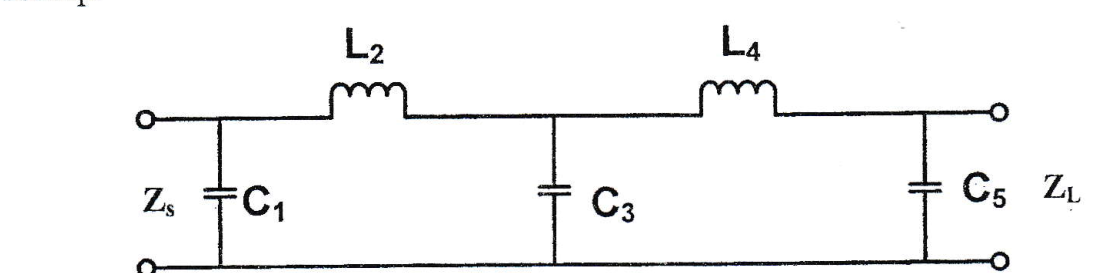
\includegraphics[width=0.62\linewidth]{figs/rf_82bh_filter.png}\hfill\mbox{}
\end{asked}
\lead{Step 1: specification (assumed, and say so)}
\begin{itemize}
  \item The ladder is shunt $C_1$, series $L_2$, shunt $C_3$, series $L_4$, shunt $C_5$: a
    \textbf{fifth-order low-pass} filter, first element shunt.
  \item Assume Butterworth, $f_c = 2.5$ GHz, $R_0 = Z_S = Z_L = 50\,\Omega$, substrate
    $\epsilon_r = 4.2$, $h = 1.58$ mm.
\end{itemize}
\lead{Step 2: prototype and Step 3: scaling}
\begin{tabularx}{\linewidth}{@{}L{1.1cm}L{1.6cm}L{4.3cm}L{1.9cm}X@{}}
\toprule
\hrow \thead{Element} & \thead{$g_k$} & \thead{Scaling} & \thead{Lumped value} & \thead{Microstrip ($Z$, $\beta l$, $W$, $l$)} \\
\midrule
$C_1$ & $0.618$ & $g/(R_0\omega_c)$ & $0.787$ pF & $20\,\Omega$, $14.2^\circ$, 11.27, 2.49 mm \\
$L_2$ & $1.618$ & $R_0g/\omega_c$ & $5.15$ nH & $120\,\Omega$, $38.6^\circ$, 0.43, 7.64 mm \\
$C_3$ & $2.000$ & $g/(R_0\omega_c)$ & $2.55$ pF & $20\,\Omega$, $45.8^\circ$, 11.27, 8.07 mm \\
$L_4$ & $1.618$ & $R_0g/\omega_c$ & $5.15$ nH & $120\,\Omega$, $38.6^\circ$, 0.43, 7.64 mm \\
$C_5$ & $0.618$ & $g/(R_0\omega_c)$ & $0.787$ pF & $20\,\Omega$, $14.2^\circ$, 11.27, 2.49 mm \\
\bottomrule
\end{tabularx}
{\color{sub}\footnotesize $\omega_c = 2\pi\times2.5\times10^9 = 1.571\times10^{10}$ rad/s. Capacitor
lines: $\beta l = g\,Z_l/R_0$; inductor lines: $\beta l = g\,R_0/Z_h$. $W$ from Hammerstad synthesis,
$l = (\beta l/360^\circ)\lambda_g$.}
\begin{itemize}
  \item \textbf{Check}: the lumped ladder gives $|S_{21}| = -3.01$ dB at 2.5 GHz (\code{filt.py}).
  \item \textbf{Step 4: implementation}: the double-$\pi$ stepped-impedance layout of $\S$6.3
    (three pads, two thin lines), with $50\,\Omega$ feeds ($W = 3.13$ mm) at both ends.
  \item \textbf{Why ILM} (3 marks): $\S$6.1.
\end{itemize}

